\documentclass[conference]{IEEEtran}

\usepackage[dvips]{graphicx}
\usepackage{amsmath,amssymb}
\usepackage{algorithm}
\usepackage{algorithmic}
\usepackage{flushend}

\renewcommand{\sfdefault}{cmss}
\renewcommand{\rmdefault}{cmr}
\renewcommand{\ttdefault}{cmtt}

\usepackage{polyglossia}
\setdefaultlanguage[babelshorthands=true]{russian}

\usepackage{fontspec}
\setmainfont{FreeSerif}
\newfontfamily{\russianfonttt}[Scale=0.7]{DejaVuSansMono}

\usepackage{caption}
\usepackage{float}
\usepackage[colorlinks,filecolor=blue,citecolor=green,unicode,xetex]{hyperref}
\usepackage{cmap}
\usepackage{amsmath,amssymb}
\usepackage[mathcal]{euscript}
\hypersetup{colorlinks=true, linkcolor=blue, citecolor=blue, filecolor=blue, urlcolor=blue, pdftitle=1, pdfauthor=, pdfsubject=, pdfkeywords=}

\sloppy
\clubpenalty=0
\widowpenalty=0
\raggedbottom

\begin{document}
\title{TRIK Studio: Technical Introduction}
\date{}%date stay empty

\author{
	\IEEEauthorblockN{Dmitry Mordvinov}
	\IEEEauthorblockA{
		Department of Software Engineering \\
		St.-Petersburg State University \\
		St.Petersburg, Russia \\
		Email: mordvinov.dmitry@gmail.com
	}
\and
	\IEEEauthorblockN{Yurii Litvinov}
	\IEEEauthorblockA{
		Department of Software Engineering \\
		St.-Petersburg State University \\
		St.Petersburg, Russia \\
		Email: y.litvinov@spbu.ru 
	}
}

\maketitle

\begin{abstract}
This paper presents TRIK Studio --- an environment for visual (and textual) programming of robotic kits, which is used in educational organizations across Russia and Europe. First part of the article provides overview of the system --- its purpose, features, differences from similar programming environments, general difficulties of robot programming and solutions proposed by TRIK Studio. Second part presents implementation details of TRIK Studio and its most interesting components. This article combines five fields of study: robotics, domain-specific visual modelling, education, formal methods and methods of program analysis. Main contribution of this article is detailed technical description of TRIK Studio as a complex and successful open-source cross-platform robot programming environment written in C++/Qt, and first part of the article can also be interesting for teachers as it provides an overview of existing robot programming tools and related problems.
\end{abstract}

\section{Introduction}
\label{chapter:intro}
Current state of school education in computer science turned out to be quite like Seymour Papert predicted it to be. In 1967 he introduced a virtual Logo turtle, that is used to teach students programming at schools even nowdays. It is less known that Papert in his experiments also used a mechanical robot turtle, that was controlled from a computer ~\cite{papert1980mindstorms}, and it made educational process much more entertaining. Today Papert's ideas are widely spread, a lot of schools are using robots to teach programming (for instance, in Russia robotics is a part of compulsory education program within the Technology course \cite{черёмухин2014внедрение,лучин2016внедрение}). Several robotics educational kits are used, including Lego Mindstorms NXT, Lego Mindstorms EV3 \footnote{LEGO Mindstorms homepage, URL: http://www.lego.com/en-us/mindstorms (accessed: 07.02.2017)}, 
TRIK\footnote{TRIK robotics platform homepage, URL: http://www.trikset.com/ (accessed: 07.02.2017)} etc.

The task of programming a robot is more complex than programming a virtual turtle: the program will be composed of manipulating motors power and sensor values instead of simple movements and turns. Therefore a lot of attention is paid to robot programming environments. Many of them are based on visual, diagram languages since they are more intuitive and easy to learn than textual ones. Programming in such visual environments is performed via drag-and-dropping blocks using mouse, and it makes programming available to small kids, that cannot even read yet. 

Popularity of visual languages in educational robotics is proven by a number of diagram-based programming environments in this field. The most known are Robolab~\cite{erwin2000lego}, NXT-G~\cite{kelly2010lego} and EV3-G~\cite{valk2014lego}, Scratch~\cite{resnick2009scratch} and Scratch-based environments (S4A~\cite{s4a}, mBlock~\cite{mblock}, Enchanting~\cite{enchanting}, ScrathDuino~\cite{scratchduino}, Blockly~\cite{blockly} and App Inventor~\cite{wolber2011app}, 12Blocks~\cite{12blocks}, Open Roberta~\cite{jost2014graphical}, Ardublock~\cite{ardublock}), less known are Robo PRO~\cite{chang2006incorporating} for programming robots created with fischertechnik robotics kits or Program Maker for Scribbler robots and several tools for preschoolers: Lego WeDo Software~\cite{mayerova2012pilot}, Create~\cite{cross2013visual}, Wonder~\cite{wonder}. 

For the last decade educational robotics has been and still is a very promising scientific field, so in 2010s almost every major university in the world invested in development of own projects in robotics. For example, in 2016 Harvard University presented Root platform~\cite{root}, Carnegie Mellon University develops and promotes its Arts\&Bots project~\cite{cross2013visual}, MIT contributed delivering Scratch environment~\cite{resnick2009scratch} and so on. Detailed overview in Russian could be found in~\cite{mordvinov2016NONPUBLISHED}, and the author concludes there that despite the variety of tools in this field there is no single one that can satisfy the needs of all educational organizations. Vast majority of such tools implement only the basic functionality (visual editor for diagrams and an ability to run programs on a robot autonomously or in a controlled manner from the computer), but they lack more advanced tools for teaching programming. Examples of such tools could be generation of readable texual code from created diagrams (that will help students to migrate from diagram-based to code-based programs), tools for debugging the program using virtual robot simulator or embedded tools for checking correctness of created programs (which could help teachers checking students' tasks). Some tools do have some of these advanced features, but often only some of them, and most of such programming environments are proprietary (which puts their users into a vendor lock-in situation) and pretty expensive for lots of schools.

Almost all aforementioned visual languages are based on control-flow computational model. Such a model is easier to understand, so it suits the purpose of education well. Nevertheless this model is not the best for programming robots since they are highly reactive by their nature: the program controlling the robot is basically a transformation of sensor signals into motor impulses. Reactive models are best expressed in data-flow languages~\cite{johnston2004advances}, where the program consists of a number of <<black boxes>>, connected with data channels. Each such <<box>> (we will call it \textit{block}) has a fixed number of inputs and outputs, and its job is to transform input data into output data (we will call data transfering through channels \textit{tokens>}). For instance, each robot's sensor is represented by a single block, that simply sends tokens with sendors data to its output. Many researchers  note usability of visual data-flow langiages comparing to texual ones~\cite{johnston2004advances}, in particular because of clear visualization of data flows.

The idea of using data-flow programming languages in robotics is not a novel one, they are implemented in almost every toolset for programming industrial and laboratory automation system. Among them are LabVIEW by National Instruments~\cite{kodosky1991visual}, Simulink~\cite{dabney2004mastering}, and Microsoft Robotics Developer Studio~\cite{jackson2007microsoft}. All of them solve the automation task very well and have very powerful tools inside (for example, Microsoft Robotics Developer Studio is run on MySpace social network servers~\cite{scherotter2009ccr}), but are very complex and hard to learn, so even if they are used in education, only in universities~\cite{stefanovic2011labview,yi2005labview}. School experiments with LabVIEW were popular in the late 1990s~\cite{cyr1997low,portsmore1999robolab}, which resulted in adaptations of this environment (like Robolab), where data-flow model was replaced with control-flow model. So, a gap between simplified languages suitable for education and more elegant, but complex industrial languages exists. Some reseachers are trying to adapt the data-flow model for educational robotics, for example a research group from New Zealand introduced the RuRu~\cite{diprose2011ruru} language. Nevertheless to our best knowledge there are still no production-ready data-flow based programming environments for educational purpose today.

Current paper describes TRIK Studio programming environment, an attempt to solve the problem	 mentioned above. The success in solving them is indirectly acknowledged by its applications: currently TRIK Studio is widely used in Russian education organizations (almost a hundred of schools and robotic clubs), several cases of TRIK Studio usage in organizations in Great Britain and France are known, there are TRIK Studio users on every inhabited continent. This paper presents technical overview of the programming environment, educational and methodical issues are not discussed in detail.

\section{General description}
\label{chapter:generalDescription}

TRIK Studio is an environment that allows to program robots using diagram-based and textual languages. It 	emerged as a further evolution of QReal:Robots~\cite{terekhov2013sreda} project, developed at Software Engineering chair of Saint-Petersburg State University. The official release supports Lego Mindstorms NXT, Lego Mindstorms EV3 and TRIK robotic kits. Each one of these kits can be programmed using one of two visual languages (the more simple control-flow and more complex data-flow language) or one of a number of texual ones. For Lego NXT the programmer can choose from NXT OSEK C and Russian version of C language (simplified for teaching textual programming), for TRIK --- JavaScript, F\#~\cite{kirsanov2014robotics} or PascalABC.NET~\cite{doliner2014basics}, for Lego EV3 the single official language for standard firmware, EV3 virtual byte code, is supported.

A program created using one of visual languages (\textit{a visual program}) could be executed in one of three modes:
\begin{itemize}
    \item debugging using virtual simulator,
    \item debugging on a PC while sending commands to a robot via USB, Bluetooth or Wi-Fi (see~\ref{chapter:communications}),
    \item textual code generation mode with subsequent upload and execution of the program on the robot.
\end{itemize}

The the first mode the program is being interpreted on a two-dimentional robot model (see Section~\ref{chapter:2dModel}). Users are able to create 2D-model of the world surrounding the robot out of walls, colored elements and floor markup. According to TRIK Studio users this feature is very useful for initial program debugging, before any interaction with real robots. Our experience shows that this virtual model editor allows to recreate most of fields and obstacle courses used in competitions in robotics. Having such a simulation environment makes possible learning robotics and programming even without having the real robotic kits. There is also an experimental support for V-Rep 3D visual simulation environment~\cite{rohmer2013v}.

Debugging using a PC (so called \textit{interpretation mode}) is useful as a next step to see how the program behaves on a robot in real time. In this mode program variables' values can be observed in a special window (similar to how it is done in Watch list windows in almost all textual IDEs) and sensor data can be displayed in a form of graphs. 

Code generation mode enables users to move from visual to textual programs. Gerenated code is displayed in an embedded QScintilla-based~\footnote{https://riverbankcomputing.com/software/qscintilla/intro (accessed: 07.02.2017)} text editor, that provides a set of common features of a code editor: syntax highlighting, code audocompletion, undo/redo, brackets highlighting etc. TRIK Studio installation contains everything neede for buiding and uploading programs into a robot (a number of cross-compilers, WinSCP, Putty, etc.), and it allows to make compilation process and communication with robots transparent to TRIK Studio users.

TRIK Studio's user interface is shown on Fig.~\ref{image:TS_interface}. It displays process of debugging a program that passes the maze using virtual simulation model.

\begin{figure*}[ht]
    \centering
    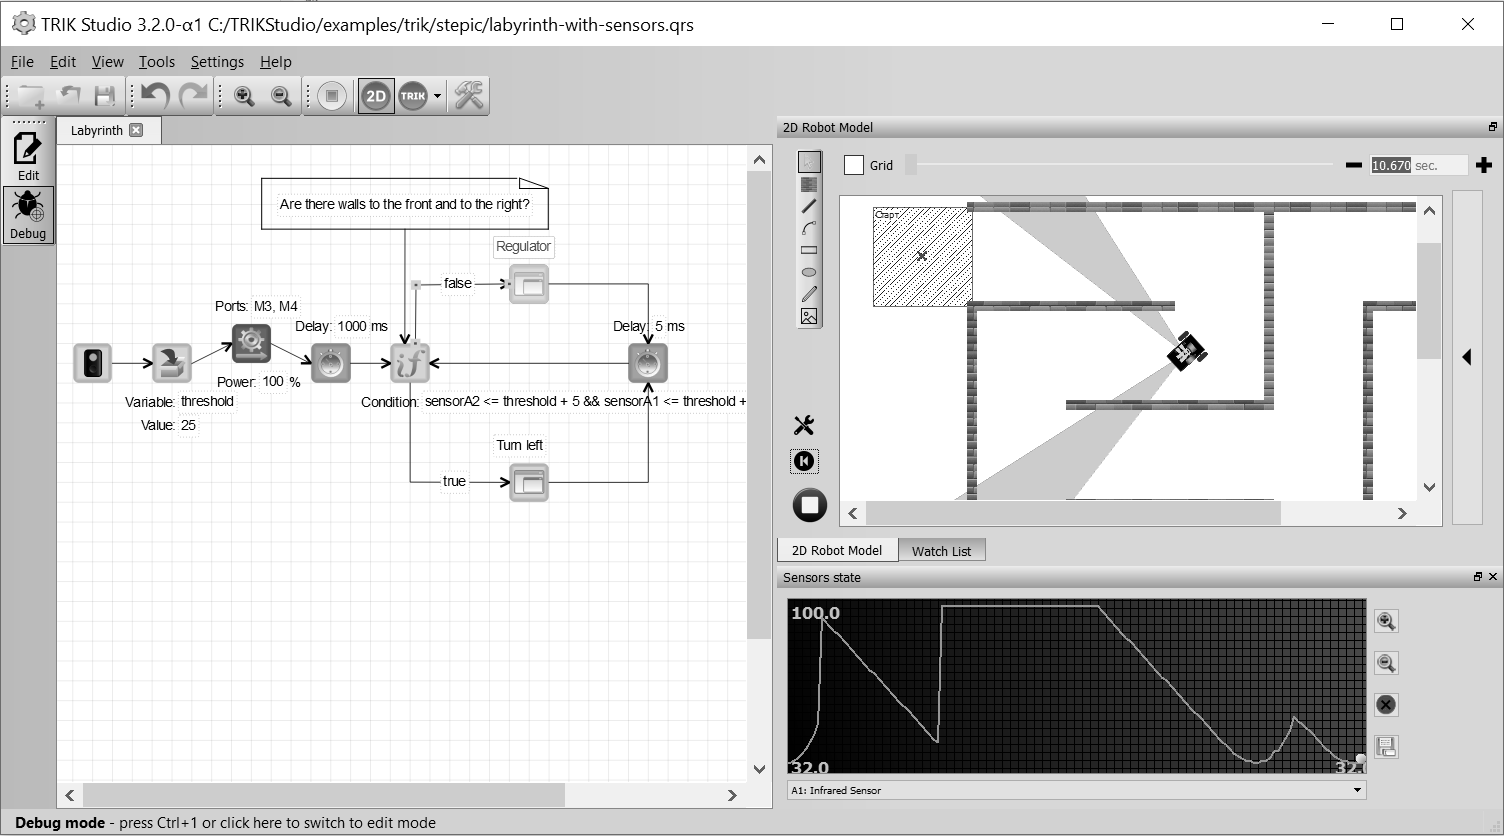
\includegraphics[width=\textwidth]{TS_CF_Labyrinth.png}
    \caption{TRIK Studio's user interface}
    \label{image:TS_interface}
\end{figure*}

In 2D simulation mode the automatic task checking feature is available (see Section~\ref{chapter:constraintsChecker}). Task checking program is written in internal event-based textual language, the file containing virtual world model and task checking program can be distributed as a task for students. Based on this feature a remote course has been launched on Stepik platform\footnote{https://stepik.org/s/7qe3xj4Z (accessed: 07.02.2017)} containing video lectures on cybernetics and robotics, numerous small tests and more that 20 tasks on educational robotics. Each task can be downloaded, solved, checked within TRIK Studio on a student's computer, and uploaded to the server where the checking system will run it on its own tests (similar to ACM ICPC coding contests).

TRIK Studio is written in C++ using cross-platform Qt\footnote{https://www.qt.io/ru/ (accessed: 14.05.2016)} framework, there are installers for Windows, Linux and Mac OS X operating systems. Because of the fact that official Lego NXT drivers are not available on Linux and Mac OS X x64, TRIK Studio contains our own implementation for them (see Section~\ref{chapter:communications} for details). The programming environment is completely free to use, open-source and is distributed under Apache License 2.0\footnote{http://www.apache.org/licenses/LICENSE-2.0 (accessed: 07.02.2017)}.

Aforementioned features distinguish TRIK Studio from all other such tools. In fact among all mentioned in Section~\ref{chapter:intro} tools only 12Blocks have a comparable feature set, but it generates complex and unreadable code (for Lego NXT), does not have tools for checking tasks, is not free to use and does not have Russian localization in it. Among the TRIK Studio drawbacks we should mention weak methodological support, limited only by embedded reference guide in Russian, a set of examaples and the remote video course. Less important drawbacks will be mentioned in the following sections. 

The rest of the paper is structured as follows. Sections~\ref{chapter:controlFlowLanguage} and~\ref{chapter:dataFlowLanguage} briefly present TRIK Studio visual languages and their interpreters. Section~\ref{chapter:commonArchitecture} overviews the system architecture. Further sections describe separate TRIK Studio subsystems. Section~\ref{chapter:communications} presents robots communication infrastructure. Section~\ref{chapter:interpreters} describes visual language interpreters. The most interesting implementation details of code generators from control-flow language are provided in Section~\ref{chapter:generators}. Section~\ref{chapter:parser} presents textual languages parsing subsystem. Section~\ref{chapter:2dModel} presents implementation details of 2D simulation model sybsystem. Section~\ref{chapter:constraintsChecker} describes task checking language and Section~\ref{chapter:conclusion} concludes the paper.

\section{Visual language for beginners}
\label{chapter:controlFlowLanguage}

The simplified control-flow based lanaguage (see Fig.~\ref{image:TS_CF_Example}) is the most often used one in TRIK Studio. It it a graph language, i.e. the program consists of nodes (\textit{blocks}) and edges, organizing the nodes into a control flow. To create a program users drag-and-drop necesary blocks onto the editor's scene, sets their properties and connects them with arrows. While being run each block executes a sequence of basic commands and passed control to outgoing edges (to all or some of them depending on the block semantics). 

All language blocks could be devided into four groups.

\begin{itemize}
    \item The first group is for blocks supporting basic algotithmic expressions, like the start and the end of a program or a subprogram, conditions, switches, arithmetic loops, blocks for execution parallelization and for working with concurrent tasks (e.g. for merging and interruprting tasks), subprogram call and a block for textual programming.
    \item The second group combines blocks working with robot peripherals. These are actions that don't require waiting. For example, they are blocks for setting motor powers, playing sounds, accessing robot video processing capabilities, synthesizing speach by given text, controlling motor encoders and LEDs, sending messages to other robots (a part of multi-agent interaction support), working with robot file system, etc.
    \item The third group consists of blocks, that <<freeze>> the control flow. They are a timer block waiting for a given number of milliseconds (similar to \texttt{msleep} function), blocks waiting for a given value from a given sensor or from an operator gamepad, and a block waiting for receiving a message from another robot. 
    \item And finally, the fourth group contains blocks that provide drawing functions for basic primitives (the drawing is being performed on a robot's screen). Such primitives are lines, rectangles, ellipses, arcs, text, images. There are parameters to change color and width of pen and brush used in drawing. There are also special blocks that control robot model marker in a 2D simulation environment. It allows robot model to leave a trace on a ground while moving, similar to the Logo turtle.
\end{itemize}

\begin{figure*}[ht]
    \centering
    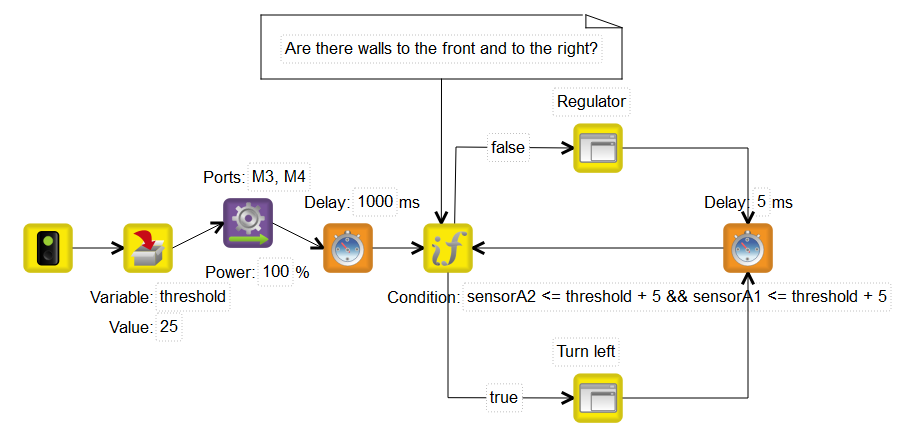
\includegraphics[width=0.8\textwidth]{TS_CF_Labyrinth_Diagram.png}
    \caption{The program of traversing the maze using right-hand rule. The first four blocks initialize the program: set the wall proximity variable, turn the robot motors on, after that the robot moves for one second to enter the maze. The second four blocks define the main control loop. Each ten milliseconds the robot checks using its infrared sensors if it can move forward or right (the \texttt{sensorA2 <= threshold \&\& sensorA1 <= threshold} condition). It it can move forward, the movement will be performed using proportional control over the right sensor data (<<Регулятор>> subprogram). If there are walls in front of the robot and to the right, it turn 90 degrees left (<<Налево>> subprogram)}.
    \label{image:TS_CF_Example}
\end{figure*}

Properties of each block can be set both within the diagram editor's scene and using special property editor window. All block properties (where applicable) support computable expressions written in TRIK Studio embedded textual language -- a statically typed Lua\footnote{http://www.lua.ru/ (accessed: 07.02.2017)} dialect. The parsing module for this parguage is written using a parser combinator library for C++11, also created within TRIK Studio project. Type inference of the resulting abstract syntax tree is performed using slightly simplified Hindley-Milner algorithm~\cite{damas1982principal}.

The domain-specific approach (\textit{DSM-approach})~\cite{koznov2008} was employed to create the described visual language. An editor was created using QReal DSM platform~\cite{qrealMeta,kuzenkova2013qreal}.  Language metamodel was defined using QReal's metaeditor, and a plugin implementing the editor was automatically generated using QReal's tools. Plugging this module into the QReal's platform core a complete visual IDE based on the given language is obtained. This IDE <<inherits>> all tools and features of the DSM platform, including modern user interface, mouse gestures recognition support for creating diagram elements~\cite{osechkina2010gestures,osechkina2012multistroke}, copy-pasting and undo/redo frameworks, zooming tools, tools for creating several types of edges on diagrams, model explorers, touch screens support and many more. According to its users TRIK Studio's user interface is much more usable and ergonomic than in any other such programming environment, and we spent about three man-days on it. We believe that it acknoledges the choice of QReal DSM platform as an underlying technology, but we have to note that while creating tool support for TRIK Studio numerous improvements were made to the QReal platform itself.

\section{Visual language for advanced users}
\label{chapter:dataFlowLanguage}

Для пользователей, освоивших программирование на языке с передачей управления, в среде существует возможность программирования на более сложном, но более удобном визуальном языке. Этот язык построен на модели потока данных (\textit{dataflow model}). В отличие от предыдущего языка, где управление в программе явно передается по стрелкам, блоки в данном языке исполняются параллельно, обмениваясь друг с другом токенами по каналам данных. К примеру, у программы на потоковом языке может быть сразу несколько точек входа (чаще всего, это датчики робота, которые посылают данные далее по цепочке их обработки), в то время как у каждой программы на языке с передачей управления есть лишь одна входная точка. Аналогично предыдущему, потоковый язык содержит блоки поддержки основных алгоритмических конструкций, блоки взаимодействия со всеми устройствами роботов, блоки рисования и т.д. Как правило, диаграммы на потоковом языке получаются лаконичнее, чем аналогичные диаграммы на языке с передачей управления. К примеру, на рисунке~\ref{image:alongTheBox_CF_DF} пропорциональный регулятор для следования вдоль стены на языке с передачей управления сопоставлен пропорционально-дифференциальному регулятору на потоковом языке.

\begin{figure}[ht]
    \centering
    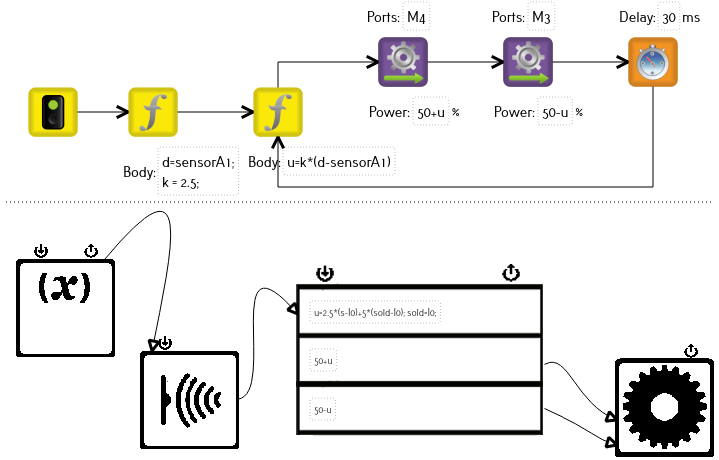
\includegraphics[width=\columnwidth]{TS_AlongTheBox_Comparison.png}
    \caption{Регуляторы на двух языках}
    \label{image:alongTheBox_CF_DF}
\end{figure}

Для упрощения изучения <<продвинутого>> языка в нем сохраняется концептуальная совместимость с моделью потока управления. Блоки здесь также могут быть выстроены в цепочку с явной передачей управления, для этого на большинстве блоков есть специальный порт активации, который игнорирует приходящие на него данные и попросту <<включает>> блок подобно тому, как это происходит в языке с передачей управления. Поначалу программирование на нем может вестись сходно с тем, как оно велось на языке для начинающих, и лишь с приходом должного опыта пользователь будет выражать свои идеи меньшим количеством блоков. 

Выразительная сила языка позволяет описывать на нем известные в робототехническом сообществе подходы к построению сложных систем управления роботов, такие как категориальная архитектура, предложенная Родни Бруксом~\cite{brooks1986robust}, архитектура <<колония>> Джонатана Коннелла~\cite{connell1989colony}, схема поведенческой навигации Рональда Аркина~\cite{arkin1987motor}, или распределенная схема навигации DAMN~\cite{rosenblatt1997damn}. Доказательство этих фактов является скорее материалом для отдельной статьи и здесь приведено не будет (при желании читатель может убедиться в этом на собственном опыте). Близкие идеи на эту тему могут быть найдены в статье английских исследователей~\cite{simpson2009toward} и диссертации~\cite{banyasad2000visual}.

Следует отметить, что на момент написания статьи поддержка потокового языка в среде реализована в экспериментальном режиме и не входит в официальную версию, распространяемую между конечными пользователями. Исходный код его редактора и инструментальной поддержки находится в открытом доступе\footnote{https://github.com/ZiminGrigory/qreal/tree/DFVPL (дата обращения: 14.05.2016)} и может быть собран вместе с исходным кодом TRIK Studio.

\section{General architecture}
\label{chapter:commonArchitecture}

Цель данной главы --- структурирование информации предыдущих разделов в виде архитектурного описания: большинство описываемых здесь деталей в каком-либо виде уже были упомянуты выше. Все диаграммы, представленные в данной главе абстрагированы от множества деталей, которые, хоть и представляют интерес в контексте данной статьи, здесь представлены не будут из соображений краткости.

На рисунке~\ref{image:commonTSArch} представлена часть общей архитектура среды TRIK Studio. Как из него видно, система разбита на несколько <<слоев>> абстракции. Каждый <<слой>> содержит код, реализующий сложные элементы функциональности среды и при этом имеет свой строго определенный и задокументированный API. На самом низком уровне такими <<слоями>> являются библиотеки взаимодействия с реальными и виртуальными роботами. На основе такого взаимодействия строится иерархия устройств робота (датчиков, приводов, дисплеев, динамиков, пультов управления, кнопок на контроллере и т.д.), из которых, в свою очередь, составляется описание модели того или иного конструктора роботов. Описания модели роботов группируются в подключаемые к ядру TRIK Studio модули, они используются другими подсистемами TRIK Studio (интерпретаторами и генераторами, которые также представляют собой подключаемые к ядру TRIK Studio модули).

Ядро TRIK Studio, в свою очередь, является подключаемым к DSM-платформе QReal модулем\footnote{Таким образом, в проекте реализована двухуровневая схема подключаемых модулей, подобно тому, как это сделано в системе ReSharper от компании JetBrains: ReSharper может расширяться подключаемыми модулями, при этом сам является подключаемым к Visual Studio модулем}. Оно подстраивает интерфейс QReal под себя, добавляя к нему множество панелей и окон, таких, как окно двумерного симулятора, панели конфигурирования датчиков робота, просмотра их значений и построения графиков и т.д.; подгружает все описания моделей роботов и отвечает за их рассылку всем необходимым подсистемам, предоставляет пользователю информацию о работе процесса генерации и интерпретации, и т.д. Наряду с ядром инструментальной поддержки TRIK Studio, к ядру QReal подключаются модули, описывающие редакторы визуальных языков, которые сгенерированы самой платформой QReal. Подробности про подсистемы более низкого уровня на рис.~\ref{image:commonTSArch} даны в главах ниже.

\begin{figure*}[ht]
    \centering
    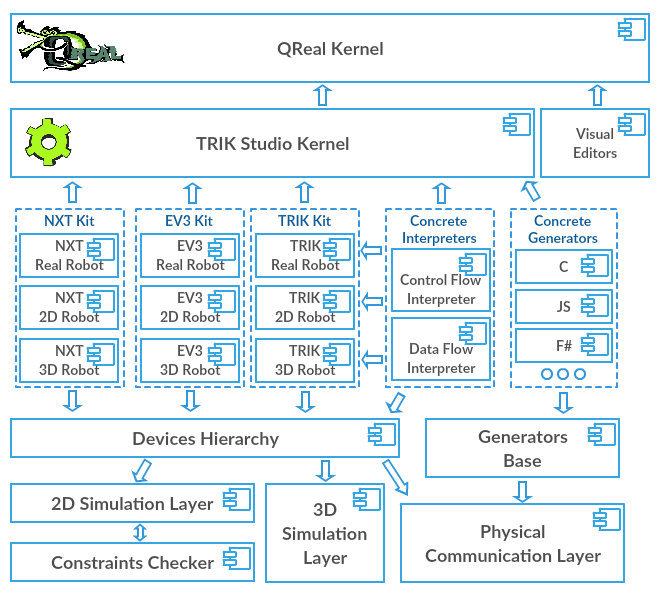
\includegraphics[width=0.6\textwidth]{TS_Common_Architecture.png}
    \caption{Общая архитектура системы}
    \label{image:commonTSArch}
\end{figure*}

Как можно заметить, вся среда построена на принципе подключаемых модулей. Отметим, что такая идея позволила сделать более гибкой систему конфигурирования установки: пользователь может выбрать, какие компоненты ему интересны, а остальные отключить (например, если у него есть только конструктор Lego EV3, то ему не нужны модули поддержки конструкторов Lego NXT и TRIK, в таком случае к нему на компьютер даже не попадут файлы, эту поддержку предоставляющие). Более того, такой подход хорошо совместим с пакетной организацией систем установки программ на различные дистрибутивы Linux. Это хорошо и с архитектурной точки зрения, так как исчезает большинство зависимостей между компонентами --- ядро TRIK Studio, к примеру, <<минималистично>>, оно <<не знает>> обо всех возможностях среды и содержит лишь общие для каждого робототехнического конструктора объекты и интерфейсы. API каждого <<слоя>> абстракции  зафиксировано и задокументировано, это может позволить создавать модули поддержки новых языков и конструкторов в среде даже независимым разработчикам из сообщества проекта.

\section{Communications with robot controllers}
\label{chapter:communications}

Одна из важных подсистем TRIK Studio --- это модуль взаимодействия с контроллерами роботов по тому или иному физическому протоколу. На рисунке~\ref{image:commonTSArch} это один из самых низких <<слоев>> абстракции среды. API модуля коммуникаций предоставляет следующие операции:

\begin{itemize}
    \item переключение текущего физического способа взаимодействия с целевым устройством (контроллером робота) между Bluetooth, USB и Wi-Fi,
    \item указание адреса устройства в терминах физического протокола (это может быть номер COM-порта в случае с взаимодействием по Bluetooth, IP-адрес или имя хоста в случае с взаимодействием по Wi-Fi),
    \item подключение-отключение к целевому устройству,
    \item посылка набора байтов на целевое устройство,
    \item события получения набора байтов с целевого устройства,
    \item события изменения статуса подключения (такие события вырабатываются, если связь с роботом установилась или разорвалась),
    \item события, оповещающие обо всех произошедших ошибках с локализованным их описанием.
\end{itemize}

Взаимодействие по USB происходит посредством библиотеки libusb\footnote{http://libusb.org/ (дата обращения: 14.05.2016)}, для реализации обмена по Bluetooth используется библиотека QextSerialPort\footnote{https://github.com/qextserialport/ (дата обращения: 14.05.2016)}, взаимодействие по Wi-Fi происходит поверх протоколов TCP и UDP посредством библиотеки QtNetwork, сложные протоколы коммуникации (такие как конфигурирование робота ТРИК перед запуском программы на исполнение) реализованы посредством Qt State Machine Framework. Процесс общения с целевым устройством происходит в отдельном потоке, чтобы не <<замораживать>> пользовательский интерфейс. Конкретные реализации механизмов коммуникации в подсистеме могут быть расширены и подменены другими компонентами <<извне>>, это используется, например, для совместимости TRIK Studio со стандартным драйвером Lego NXT. Отметим, что взаимодействие через него --- это не единственный способ общения с контроллером NXT по USB в TRIK Studio, в среде реализован собственный драйвер взаимодействия с Lego NXT, однако, в отличие от официального, работающий на всех поддерживаемых операционных системах через libusb.

\section{Interpreters}
\label{chapter:interpreters}

Интерпретатор преобразует визуальную диаграмму в последовательность команд на целевом устройстве (рис.~\ref{image:interpretersTSArch}). При этом иерархия устройств в системе построена таким образом, что не делается различий, реальное ли это устройство или симулируемое (рис.~\ref{image:devicesTSArch}). Каждое устройство представляет собой класс C++, содержащий код взаимодействия с целевым механизмом. Реализации устройств какого-либо конструктора находятся в соответствующих библиотеках подключаемых модулей. Для общения по физическим каналам устройства используют подсистему коммуникаций (гл.~\ref{chapter:communications}), для передачи команд двумерному и трехмерному симуляторам --- API этих симуляторов.

\begin{figure}[ht]
    \centering
    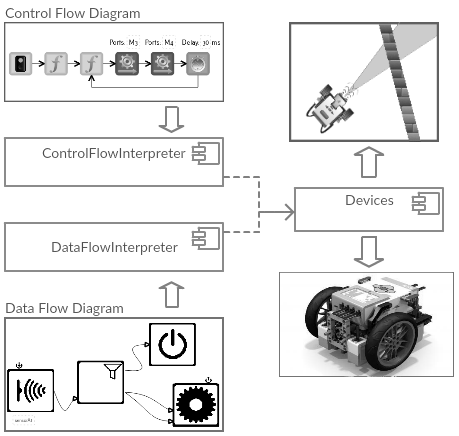
\includegraphics[width=0.9\columnwidth]{TS_Interpreter_Architecture.png}
    \caption{Общий принцип работы систем интерпретации}
    \label{image:interpretersTSArch}
\end{figure}

\begin{figure*}[ht]
    \centering
    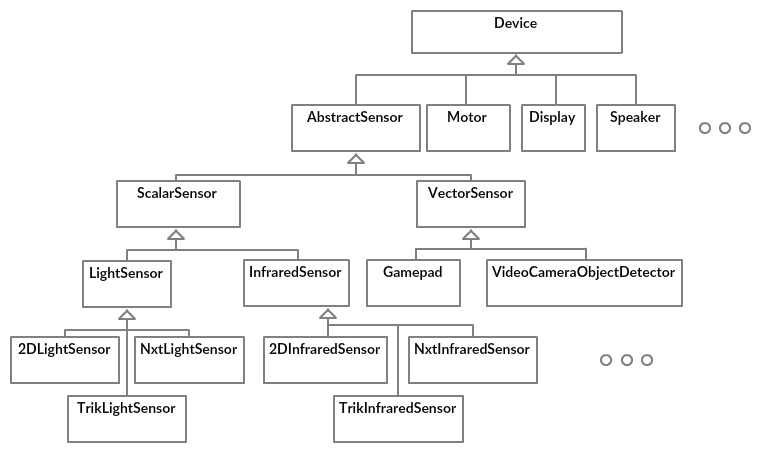
\includegraphics[width=0.7\textwidth]{TS_Devices_Architecture.png}
    \caption{Часть иерархии устройств в системе}
    \label{image:devicesTSArch}
\end{figure*}

Интерпретаторы, также как и вся система в целом, написан на языке C++ с использованием инструментария Qt. На вход подсистеме интерпретации поступает
описание созданной пользователем диаграммы в некотором внутреннем представлении. В среде реализовано два интерпретатора: интерпретатор языка для начинающих с передачей управления и интерпретатор потокового языка.

Интерпретатор первого языка находит на диаграмме начальный блок, и далее трассирует поток управления диаграммы в том порядке, как он задан стрелками. Текущий блок исполнения подсвечивается на визуальной диаграмме, чтобы пользователю был виден прогресс исполнения. Для каждого посещенного блока специальные фабрики интерпретатора создают объекты, которые реализуют его поведение. В общем случае, такой объект-реализация ищет среди готовых к работе устройств робота необходимые ему, вызывает соответствующие команды и передает управление следующим блокам по какой-либо исходящей ветке (которая определяется, опять-таки, самой реализацией блока). При этом не делается различий, является ли найденное устройство частью реального робота или симулируемым, таким образом, одна и та же подсистема интерпретации используется для исполнения диаграммы в двух режимах из трех (гл.~\ref{chapter:generalDescription}).

Если на каком-то шаге интерпретации повстречался блок распараллеливания, интерпретатор запускает новые потоки исполнения с соответствующих точек, создавая для каждого свой стек вызовов. Если встретился вызов подпрограммы, вычисляются ее параметры, укладываются на текущий стек вызовов, и далее процесс интерпретации повторяется рекурсивно. При достижении любого завершающего блока со стека снимается верхний фрейм, и исполнение продолжается с соответствующей точки на предыдущей диаграмме. Если при снятии очередного фрейма стек вызовов стал пустым, текущий поток исполнения считается завершенным. Таким образом, программа исполняется по мере того, как она <<открывается>> интерпретатору.

Отличительной чертой такой реализации является тот факт, что все изменения, вносимые пользователем на диаграмму во время процесса интерпретации, <<подхватываются на лету>>. Это является удобным, например, в случае подбора коэффициентов пропорциональности какого-либо регулятора, реализованного в программе. При этом процесс исполнения не изменившихся частей диаграммы оптимизирован: объекты-реализации блоков кэшируются в отдельную таблицу, то же происходит с абстрактными синтаксическими деревьями и информацией о выводе типов выражений на текстовом языке. Таким образом, если содержимое программы не меняется во время процесса интерпретации, повторная передача управления в ветки программы повлечет использование уже созданных сущностей. Валидация диаграммы также осуществляется <<на лету>>, в случае, если в диаграмме найдено некорректное место, пользователю отображается локализованное сообщение об ошибке. Последняя черта может рассматриваться как отрицательная, так как сообщение об ошибке появляется лишь в момент ее достижения в программе, что, впрочем, типично и для широко используемых текстовых интерпретируемых языков.

Интерпретатор потокового языка работает в два этапа. На первом, подготовительном этапе диаграмма проходит валидацию, создаются объекты-реализации элементарных блоков, преобразующие диаграмму в команды на устройствах роботов подобно тому, как это происходит в интерпретаторе языка, описанного в предыдущей главе. Объекты-реализации соединяются друг с другом посредством механизма сигналов и слотов инструментария Qt в соответствии с тем, как они соединены потоками данных на диаграмме; здесь оказался полезным паттерн проектирования <<издатель-подписчик>>. На втором этапе интерпретатор запускает на автономное исполнение каждый из блоков, в который не входит ни один поток данных, каждый из которых, в свою очередь, будет активировать блоки, соединенные с ним выходными потоками данных при выработке токенов. Исполнение блоков происходит псевдопараллельно с централизованной очередью сообщений (рис.~\ref{image:dsPseudoparallelism}). Это решение отличает данный язык от всех его промышленных аналогов (к примеру, в Microsoft Robotics Developer Studio диаграмма разворачивается в набор независимых веб-сервисов~\cite{jackson2007microsoft}), его причины состоят в узкой направленности языка на <<слабые>> контроллеры учебных роботов, в которых параллельное исполнение большого количества блоков затруднительно или вовсе невозможно. Тем не менее, в языке все же присутствует блок распараллеливания, который полезен, например, для выражения вышеупомянутых подходов к проектированию сложных систем управления. Такой блок может рассматриваться как механизм низкоуровневого управления вычислительными ресурсами в языке.

\begin{figure}[ht]
    \centering
    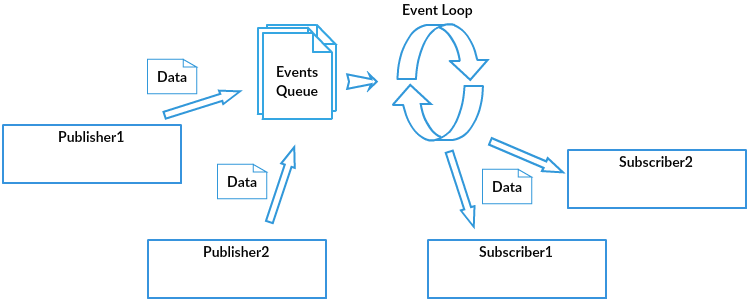
\includegraphics[width=\columnwidth]{DF_Interpretation_Process.png}
    \caption{Механизм исполнения потоковой программы в TRIK Studio}
    \label{image:dsPseudoparallelism}
\end{figure}

\section{Generators}
\label{chapter:generators}

Одна из наиболее важных и востребованных функций среды TRIK Studio --- генерация читаемого кода по визуальной диаграмме. По одной и той же диаграмме может быть сгенерирован код на любом поддерживаемом средой текстовом языке (C, JavaScript, F\#, Pascal, РуСи~\cite{тереховотечественные}, байткод ВМ EV3). Под визуальными диаграммами в данном разделе будем подразумевать программы на языке для начинающих (с передачей управления), под генераторами --- модули генерации кода по визуальным диаграммам именно этого языка.

Визуальная диаграмма состоит из блоков и стрелок, таким образом, описывает \textit{граф потока управления} программы~\cite{steven1997advanced}. Все основные алгоритмические конструкции (развилки, циклы, конструкции выбора и т.д.) складываются из стрелок. Например, чтобы задать бесконечный цикл, достаточно лишь провести стрелку от блока к одному из предыдущих, для описания циклов вида \texttt{while-do}, \texttt{do-while} или с инструкцией \texttt{break} внутри тела достаточно лишь провести одну из веток развилки из тела цикла к соответствующему блоку вне его. Очевидно, что одна стрелка на диаграмме соответствует инструкции \texttt{goto} в коде. Однако код, содержащий инструкции \texttt{goto} весьма труден для чтения человеком, тем более не подходит для обучения азам текстового программирования, поэтому следует избегать их появления в сгенерированном коде. Тем не менее, на TRIK Studio возможно написать программу, не выразимую общепринятыми алгоритмическими конструкциями, в таком случае появления инструкций \texttt{goto} в коде не избежать (существуют методы автоматического преобразования программы с goto в структурную программу, но результат их работы не лучше с точки зрения обучения текстовому программированию). С другой стороны, далеко не все современные текстовые языки поддерживают инструкцию \texttt{goto} (например, в языке JavaScript такой поддержки нет). Будем называть \textit{приводимыми} диаграммы, которые можно выразить стандартными алгоритмическими блоками (\texttt{if-then}, \texttt{if-then-else}, \texttt{while-do loop}, \texttt{do-while loop}, \texttt{while-break loop}, \texttt{switch}), код на текстовом языке, соответствующий структурированной диаграмме также будем называть \textit{структурированным}. В противном случае будем говорить, что диаграмма \textit{неприводима}, а код будем называть \textit{неструктурированным}. В случае, если диаграмму не удается сгенерировать в структурированный код, пользователю должно быть показано предупреждение.

Таким образом, реализация системы генераторов в TRIK Studio потребовала решения двух нетривиальных задач, которые сформулированы ниже в виде требований.

\begin{itemize}
    \item Система генераторов должна быть организована таким образом, чтобы добавление в систему генератора в новый текстовый язык занимало минимальное количество времени и усилий. По возможности, это должно быть по силам даже людям, не знакомым с кодом системы.
    \item Для каждого языка (где это возможно) система должна поддерживать два режима генерации: приводимые диаграммы должны быть сгенерированы в структурированный код, неприводимые --- в неструктурированный. При этом успешность структурирования диаграммы не должна зависеть от ее размера и сложности.
\end{itemize}

Первая задача является чисто архитектурной. Ее решение представлено на рисунке~\ref{image:generatorsArchitecture}. Основная идея --- разделение процесса генерации на два этапа. На первом диаграмма преобразуется в представление, независимое от целевого языка генерации --- \textit{семантическое дерево}. Семантическое дерево упорядочивает структуру графа потока управления до <<древесной>>, в независимости от того, является ли диаграмма приводимой или нет. В случае, если диаграмма приводима, родительский узел семантического дерева всегда соответствует блоку вычислений в целевом коде, дети --- инструкциям этого блока, среди которых нет \texttt{goto}. Опишем последовательность действий, отображенных на рисунке~\ref{image:generatorsArchitecture}.

\begin{figure*}[ht]
    \centering
    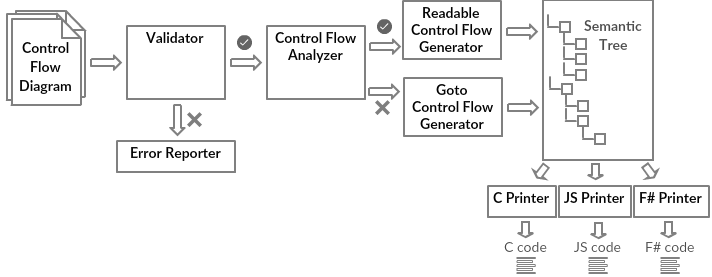
\includegraphics[width=0.6\textwidth]{TS_Generators_Architecture.png}
    \caption{Архитектура подсистемы генерации кода в TRIK Studio}
    \label{image:generatorsArchitecture}
\end{figure*}

На вход генератору поступает визуальная диаграмма. На первом этапе диаграмма обходится в глубину компонентой-валидатором (построенной с применением шаблона проектирования <<посетитель>>). Для всех выражений на встроенном текстовом языке в свойствах блоков происходит их синтаксический разбор и вывод типов. В случае, если диаграмма или код в свойстве содержит ошибки, о них сообщается пользователю в локализованном виде и процесс завершается. В случае, если диаграмма синтаксически корректна, она поступает на вход анализатору потока управления, о котором будет рассказано ниже. В зависимости от того, может ли диаграмма быть сгенерирована в структурированный код, выбирается промежуточный генератор независимого представления, который извлекает семантическое дерева из потока управления диаграммы. Если целевой язык не поддерживает инструкцию \texttt{goto} или, наоборот, высокоуровневые конструкции, как, например, ассемблер-подобный байткод ВМ EV3 (что указывается в конфигурации генератора), соответствующему генератору будет предпочтена его альтернатива. Наконец, на последнем шаге процесса генерации семантическое дерево печатается в целевой текстовый язык. Для этого используется подход с заданием шаблонов генерации для целевого текстового языка. Все, что необходимо сделать для реализации нового генератора --- переопределить набор этих шаблонов и указать конфигурацию генератора. К примеру, шаблон генерации условного оператора в язык C выглядит следующим образом: \begin{verbatim}
    if (@@CONDITION@@) {
        @@THEN_BODY@@
    } else {
        @@ELSE_BODY@@
    }
\end{verbatim}

Вторая из решенных проблем --- модуль анализатора потока управления. В терминах текстовых языков задача звучит так: по данной программе, поток управления которой описан исключительно инструкциями \texttt{goto}, требуется выдать эквивалентную структурированную программу. Данная задача решалась различными исследователями, работающими в области декомпиляции программного кода~\cite{steven1997advanced,деревенец2009структурный}. Приемлемый способ ее решения по методу \textit{интервального анализа} графа потока управления описан, к примеру, в монографии~\cite{steven1997advanced}. Алгоритм интервального анализа графа потока управления диаграммы с незначительными модификациями реализован в TRIK Studio. Коротко опишем его.

Неформально говоря, \textit{интервал} --- это участок графа потока управления с одним входом и одним выходом. Целью алгоритма является построение дерева вложенности интервалов графа потока управления программы, которое в нашем случае и является семантическим деревом. Алгоритм работает на рекурсивном подъеме поиска в глубину в графе потока управления. На каждом шаге алгоритм пробует сопоставить подграф, выходящий из текущей вершины, с каждым из шаблонов элементарных интервалов (алгоритмических конструкций, в терминах которых и будет структурирована программа). Если такой шаблон удается найти, весь подграф сворачивается в одну вершину, и процесс продолжается. Самый простой пример такого шаблона --- два интервала, соединенные ровно одной дугой, что соответствует последовательной композиции. Если на каком-то шаге ни один шаблон не подошел, то диаграмма считается неприводимой.

Очевидным ограничениям на целевой язык в текущей реализации генераторов является его императивность: цепочка блоков на диаграмме должна преобразовываться в последовательное исполнение утверждений в текстовом языке, что проще всего достигается применением оператора последовательной композиции. Тем не менее, идея использования промежуточного шага генерации в независимое представление работает и здесь. К примеру, для поддержки генерации в чисто функциональные языки достаточно расширить элементы независимого представления конструкцией продолжения (continuation passing style, CPS) и добавить промежуточный генератор диаграммы в независимое представление в форме CPS. После этого достаточно переопределить шаблоны печати независимого представления во все необходимые языки.

\section{Textual language parser and interpreter}
\label{chapter:parser}
TRIK Studio uses visual languages for robots programming, but arithmetic expressions, intrinsic function calls and so on are better represented with textual strings (in fact, NXT-G tries to use visual blocks even for arithmetic expressions, representing them as syntax trees, it is very inconvenient). As a textual part of a language for both visual languages TRIK Studio uses a subset of Lua 5.3\footnote{https://www.lua.org/}, customized for our needs. Decision to implement our own parser and interpreter of a textual language was made under these considerations:
\begin{itemize}
	\item we needed a small textual language with lightweight syntax and without explicit typing since it shall be used by non-programmers;
	\item we needed explicit abstract syntax tree and the ability to run type inference on it since we were going to generate code on C or EV3 bytecode, which is strongly typed;
	\item we needed to be able to customize language syntax if the need will arise;
	\item all existing implementations for such languages had interpreter without access to a syntax tree or a parser that was not reusable from C++ code;
	\item since we needed only a subset of a language (arithmetic expressions, without statements, custom function and type definitions), writing custom parser was not a difficult task.
\end{itemize}

Parser and interpreter were implemented as a separate library in QReal core, so the resulting textual language is available not only in TRIK Studio, but in all other domain-specific solutions based on QReal. Parser implementation consists of two parts --- general-purpose parser combinator library and Lua parser library implemented using parser combinators. Many projects use ANTLR\footnote{http://www.antlr.org/}, boost.spirit\footnote{http://boost-spirit.com/home/}, yacc\footnote{http://dinosaur.compilertools.net/yacc/} as tools for parser development, but we once again created our custom solution, mainly to avoid additional external dependencies and complication of a build process --- QReal and TRIK Studio are developed by a large community, and not everyone is happy to install additional tools and learn how to use them, especially if their work has nothing to do with syntax analysis and they are students who do not took formal languages course yet.

QReal parser combinator library supports recursive-descent parsers which are able to parse a subset of LL(1) grammars. FOLLOW($\alpha$) set is not calculated, so it limits the expressiveness of resulting grammars, but we were still able to use Lua 5.3 grammar almost as it is specified, with only minor modifications related to factorization and left recursion elimination, which shall be done anyway for LL parsers. For arithmetic expressions Precedence Climbing\footnote{http://www.engr.mun.ca/\~theo/Misc/exp\_parsing.htm} algorithm was used, and it also required some minor alterations in Lua grammar. Custom modifications were made mainly on lexer level to allow, for example, to use '!=' for inequality in addition to '\verb|~=|' used in Lua. Here is a quick example\footnote{full specification of our parser with many irrelevant technical details see at https://github.com/qreal/qreal/tree/master/qrtext/src/lua} of production written in C++ with our library ("`statement is ';' or a list of expressions, optionally followed by '=' and other list of expressions"'):
\begin{verbatim}
	// stat ::= ‘;’ | explist [‘=’ explist]
	stat = (-LuaTokenTypes::semicolon 
	    | (explist & ~(-LuaTokenTypes::equals & explist)))
\end{verbatim}

\verb|LuaTokenTypes::semicolon| is a token corresponding to ';', operator '-' creates a simple parser that can parse only semicolons and excludes semicolon from AST, "`explist"` is a reference parser object, like "`stat"', defined elsewhere, '\&' combines two parsers into a parser which accepts concatenation of their corresponding strings, '|' combines two parsers into a parser that accepts alternative, '\verb|~|' creates optional parser from its argument, which shall also be a parser. There are also operators for adding semantic actions to productions and assigning parser a name for debug purposes. When all parsers are combined in such a way, it is enough to call 'parse()' method of a resulting parser object, giving it a token stream. Parser combinator library was used for another language in QReal~\cite{tikhonova2015generation}, so it is general enough to support not only Lua.

Parser returns abstract syntax tree on which type inference algorithm is executed, providing types for all variables and expressions. Type inference uses Hindley-Milner-style~\cite{damas1982principal} algorithm, simplified for performance reasons and extended to support overloading and coercion. Type inference is also generalised and Lua type inferer only defines inference rules for Lua-specific AST nodes, core type inference functionality is available for all QReal textual languages.

After type inference is complete, expression is ready to be evaluated by an interpreter. Interpreter allows to register intrinsic functions, also it allows to add custom variables with their values, to support using current sensor values in calculations --- robot communication subsystem receives telemetry data from a robot and injects sensor readings into interpreter, which uses them to calculate expressions.

Last notable feature of parsing/interpreting subsystem is extensive use of caching to avoid parsing or reevaluating expressions as much as possible. Program shall be interpreted in real-time, so reparsing and reevaluating expressions every several milliseconds, as required by many control algorithms, would be severe performance problem. But program can be changed by user during interpretation, values for some variables may be changed by external code, such as sensor readings changed by communication subsystem --- so the interpreter keeps track of changes and uses previously calculated values if possible.

\section{Simulator}
\label{chapter:2dModel}

Особая часть среды TRIK Studio, отделимая от всей остальной системы --- подсистема двумерного имитационного моделирования робота (двумерный симулятор). Окно симулятора встроено в интерфейс TRIK Studio, но может и использоваться отдельно. Основная часть симулятора --- редактор модели мира. В специальном меню можно выбрать инструмент рисования (подобно тому, как это происходит в большинстве графических редакторов). Инструменты рисования делятся на стены (твердые предметы, на которые реагируют ультразвуковые и инфракрасные датчики роботов и сквозь которые робот не может проехать) и цветные маркеры на полу (элементы, на которые реагируют датчики цвета, освещенности и эмуляторы систем видео-зрения) --- прямые линии и кубические кривые безье, прямоугольники, эллипсы и стилус (произвольная растровая фигура, рисующаяся мышью как карандашом). Для каждого маркера на полу может быть задана его толщина, цвет и заливка. Модель робота всегда присутствует на сцене редактора мира, на ней произвольным образом можно размещать виртуальные датчики. Робот представляет собой двухколесную тележку с дифференциальным приводом. Для удобства регионы сканирования датчиков расстояния подсвечиваются. На отдельной панели для каждой поддерживаемой модели робота (NXT, EV3 или TRIK) присутствует эмулятор панели контроллера: фронтальное изображение его лицевой панели с кнопками, нажатие мышью на которые эмулирует нажатие на кнопку реального контроллера, цветными светодиодами, меняющими свой цвет соответственно тому, как того требует написанная пользователем программа, и эмулятором дисплея, изображение на котором можно менять блоками из группы <<Рисование>>.

Важной особенностью симулятора является то, что режим исполнения программы неотличим от режима создания модели мира. Модель мира может редактироваться даже в момент исполнения программы, на любое добавление пользователем стенок и цветных элементов во время исполнения программы датчики начнут реагировать немедленно; положение и направление робота и его датчиков в пространстве может быть изменено в любой момент, что соответствует в реальном мире физическому воздействию на корпус робота.

Симулятор построен на основе архитектуры Model-View-Controller. Модель содержит сериализуемое описание мира и робота, уведомляет о любом изменении любого свойства любого предмета. На события модели подписывается представление, все изменения в модели автоматически отображаются на сцене и панелях симулятора. Пользовательские действия в представлении выполняются через контролирующую компоненту, которая кладет очередное действие на вершину специального стека для возможности его отмены и повтора.

Важной частью модели является ее <<физика>>. В симуляторе реализовано две физические модели поведения робота: идеальная и реалистичная. В идеальной физике игнорируются силы трения о пол и стены, импульсы моторов, при неизменных скоростях моторов робот будет двигаться равномерно (без ускорения и замедления). Любое, даже самое легкое столкновение со стеной в такой модели остановит робота. В реалистичной модели ведется полный учет сил тяги и трения робота о пол и стены, при столкновении со стеной робот поведет себя подобно тому, как это происходит в реальности. Переключение между физическими моделями происходит при выставлении соответствующего флага на панели настроек симуляции и может произойти даже во время исполнения программы. Имеется возможность <<зашумления>> показаний датчиков и импульсов на моторах гауссовым шумом.

Время в двумерном симуляторе не соответствует процессорному: в нем существует централизованная временная прямая, темп хода которой может меняться на специальной панели (что не меняет поведения робота). Та же самая временная прямая используется в интерпретаторах визуальных языков TRIK Studio для соответствия блоков работы со временем модельному, а не процессорному времени.

\section{Automatic checking of solution correctness}
\label{chapter:constraintsChecker}

Last important subsystem which is described in this paper is automatic checker of constraints for TRIK Studio programs. This system allows to turn a world model in a simulator to an exercise with specified success and failure conditions, which can be shared among students and solutions (in a form of visual programs) can be automatically checked against these success conditions in simulator, thus providing feedback without an intervention from a teacher. To create an exercise one needs to specify two things:

\begin{itemize}
    \item what parts of a simulated worlds are fixed and can not be changed by a student (walls and figures on a floor, robot starting position, sensors and their orientations and so on);
    \item program on a special constraints definition language which specifies success and failure conditions for a solution.
\end{itemize}

Constraints are described on a special XML-based definition language. Program on this language is a set of events $\{ e_1, e_2, ..., e_n \}$, where each event $e_i$ is a triple $(id_i, c_i, T_i)$:

\begin{itemize}
    \item $id_i$ --- event id: internal label by which other parts of a program may refer to this event, can be empty;
    \item $c_i$ --- condition, under which the event is raised, a formula in a first-order predicate calculus without quantification;
    \item $T_i$ --- ordered set of triggers $[ t_{i_1}, t_{i_2}, ..., t_{i_n} ]$. Each trigger specifies an action that shall be done when event condition $c_i$ becomes true.
\end{itemize}

Each event is specified by its XML node in a program. Event can be specified in a \textit{canonical} form, or in a form of a \textit{constraint}. Event in canonical form --- already described triple $(id_i, c_i, T_i)$. Event in constraint form is a triple $(id_j, c_j, message_j)$. Constraint is interpreted as an event $(id_i, $$\neg$$c_i, [ fail(message_j) ])$, where $fail(message_j)$ --- trigger that stops simulation and reports error message $message_j$. In other words, constraint in an event that is raised when given condition is violated and reports this violation to an user. Events in a form of constraints are added to a language for pragmatical reasons only, because it is much more convenient to specify conditions like "`robot $x$ shall not leave area $a$"' or "`robot $x$ shall have a set of sensors $s$ connected"' as constraints instead of events. Special case of such constraint --- time limit. Time limit shall be specified for each constraint definition program so that constraints checker will not run simulation indefinite amount of time if all constraints are satisfied but success event is never triggered. Checker verifies that time limit is set before execution of program, and if not, considers it as semantic error.

Let's briefly describe predicates,functional symbols and elementary triggers used in a language. Predicate symbols can be divided into these groups.
\begin{itemize}
    \item Comparison predicates $>$, $<$, $\leq$, $\geq$, $=$, $\neq$.
    \item Spatial predicates. They have form "`item $x$ is located inside area $y$"'.
    \item Event state predicates $settedUp(id_i)$ and $dropped(id_i)$, denoting active and inactive events accordingly. Active events can be raised when their corresponding condition is satisfied, events in inactive state will not be raised (and their triggers will not be executed) even when condition is satisfied.
    \item Time predicate $timer(t)$, which is initially false, becomes true after $t$ ticks of model time and stays true afterwards.
    \item Other predicates that can be expressed by already described predicates, they are introduced for pragmatical reasons only.
\end{itemize}

Functional symbols can be the following.
\begin{itemize}
    \item Constants of different types (integer, floating-point, string, colour, geometrical and so on).
    \item Symbol $variableValue(id)$ that denotes a value of a variable with identifier $id$. Variables are internal to the constraints checking program (i.e. do not represent simulation state) and can be useful for implementing complex conditions like counting of times that robot does some action.
    \item Arithmetical and geometrical operations over other values --- absolute value of a number, for example, or a distance between two points.
    \item Comparison of forms of two figures using Levenshtein distance. It is useful to compare images drawn on robot display to an ideal image specified in exercise.
    \item Symbol $objectState(path)$ allows to get state of a simulated robot devices or objects of a simulated world. $path$ argument shall contain a path to a desired property in a hierarchy of objects in world model. Such path will be translated into a sequence of C++ object property references using Qt Reflection mechanism, so this symbol provides a bridge between constraints definition and simulator.
\end{itemize}

Finally, elementary triggers can be the following:
\begin{itemize}
    \item $success$, $fail(message)$ control checker state. First trigger reports exercise as successfully checked, second reports error and marks simulation result as a failure;
    \item triggers that set variable values and change properties of a simulated world or a robot devices (complementary to $objectState$ function), they allow, for example, to set random number generator seed to make possible testing of solution which uses random number generator;
    \item triggers that control event state --- every state can activate or deactivate every other state (including itself), it allows to specify rather complex checking scenarios, like visiting waypoints in a correct order within given amount of time.
\end{itemize}

An example of a simple program in constraints description language is given in~\ref{code:constraints}.

\captionsetup[figure]{name=Listing}
\setcounter{figure}{0}

\begin{figure*}[!t]
\begin{verbatim}
<!-- Root element, contains all constraints -->
<constraints>

    <!-- Mandatory time limit constraint -->
    <timelimit value="2000"/>

    <!-- Constraint on robot location -->
    <constraint failMessage="Robot left the allowed area!">
        <inside objectId="robot1" regionId="myspace"/>
    </constraint>

    <!-- Success criteria for a program: robot must say "Hello" using speech synthesis 
		     and draw a smile on a screen -->
    <event settedUpInitially="true">
        <conditions glue="and">
            <equals>
                <objectState object="robot1.shell.lastPhrase"/>
                <string value="Hello"/>
            </equals>
            <equals>
                <objectState object="robot1.display.smiles"/>
                <bool value="true"/>
            </equals>
        </conditions>
        <trigger>
            <success/>
        </trigger>
    </event>

</constraints>
\end{verbatim}
\caption{Example of constraints specification in TRIK Studio simulator model.}
\label{code:constraints}
\end{figure*}

Architecturally constraints checking system is a standalone module which uses TRIK Studio core and simulator model as shared libraries. Simulator model and robotic kit support in TRIK Studio are frequently extended with new devices, options and features, so Qt Reflection mechanism is used to access objects and their properties from constraint specifications. It allows to extend TRIK Studio core without modifications in constraints checking system itself, new properties immediately become available from constraints description language. Constraints checker subscribes to events from simulation model as another view (in MVC pattern sense) and checks constraints on every tick of model time. It may seem very ineffective, but only active constraints are checked and only a few constraints are active at any given time, so a simulation with constraints checking has almost the same performance as without it.

Described language proven to be quite effective at specifying spatial and temporal constraints on a system state. It is more expressive than, for example, temporal logic or topological temporal logic languages which are used for specification of formal constraints on robot behaviour in recent works~\cite{mordvinov2016formal,kress2007s,бугайченко2007разработка,дмитриев2013адаптация}. And this language is not Turing-complete (for example, it can not express Markov algorithms due to absence of means to work with arbitrary length collections, so it can not express string replacement), it opens a possibility to statically analyse non-trivial properties of programs on it. In addition to this, a subset of a language can be used for specification of requirements for a program to be used in formal verification. Plans for next versions of TRIK Studio include creating visual editor for constraints, which, combined with some verification engine, will possibly allow to formally prove correctness of visual programs without the need to actually write temporal logic formulae. Investigation of this idea is a promising future work direction.

Constraints checking system is also used for functional testing of TRIK Studio on continuous integration server. More on this (and other details of TRIK Studio testing) see in~\cite{mordvinov2016testing} (in Russian).

This functionality is also used as an automatic checker of exercises for MOOC on Stepik platform\footnote{https://stepik.org/s/7qe3xj4Z}. Without such checker it would be impossible to provide feedback to possibly large number of students, making course much less interactive. From a technical point of view checker is a set of scripts which launch "`headless"' interpreter (i.e. interpreter without GUI) on a correct field with correct constraints. Checker is hooked up into Stepik infrastructure and runs in a separate Docker\footnote{https://www.docker.com/} container when new solution is submitted. Checker has several fields and corresponding constraint descriptions for each task (from one to five), each solution is checked against all those fields to test that it works in different situations and is not hardcoded. Fields are hidden from the user but error reporter output does gets displayed, so students can guess what went wrong (well, theoretically. But it's better than traditional ACM ICPC system, where only a number of incorrect test and a general type of error are reported).

Checker can also send a visual representation of a field with a trace of a robot to a client. Trace consists of points of a robot trajectory and values reported by its sensors, and this trace can be played back by a web application described in~\cite{zakharov2016web} (in Russian). This web application also allows to actually create solutions for almost all tasks from the course right in the browser, form a correct TRIK Studio save file and run it on a server on checker, playing back the result, so a student perceives this as "`TRIK Studio in a browser"'. This application works standalone, but is not integrated into Stepik course yet due to technical difficulties related to Stepik infrastructure.

\section*{Conclusion}
\label{chapter:conclusion}

Technical description of TRIK Studio robots programming system was presented. TRIK Studio now has about ten thousand users across the globe, according to Google Analytics data. Now it supports English, Russian and French languages. It is open source\footnote{https://github.com/qreal/qreal (accessed: 08.02.2017)} and has large and active community developing it. TRIK Studio has about 100K lines of code (excluding QReal core, which also has size of about 120K LOC), written in C++ with Qt.

Future work consists of two major development vectors: improvements of an existing system and new research projects based on it. Improvement tasks are gathered from teachers, pupils and students which use TRIK Studio, and there is already several hundreds of such tasks tracked. For example, support for new robotic platforms (such as Arduino, STM32), improvements for simulator (more precise physics simulation, multiagent systems simulation and so on), support for more textual languages (like Python, Pascal). Research projects that are currently using TRIK Studio as a technical base include research in domain-specific visual languages field and formal methods field of study. For example, we are creating technology to automatically generate visual domain-specific language using metainformation from packages of robotic middleware (ROS~\cite{quigley2009ros} is currently considered), that visual language will be able to link middleware nodes together thus configuring environment for a particular robot. Research in formal methods aims to formalize semantics of used visual languages to be able to apply formal verification and synthesis methods to diagrams.

\bibliographystyle{utf8gost705u}
\bibliography{trikStudioEnglish}

\end{document}